% =====================================================================================
% The Variational Quantum Eigensolver (VQE) - from eigenvalue problems to a CUDA-Q implementation
% Build:  python make_figures.py   (needs cudaq, numpy, scipy, matplotlib, pyscf, openfermion, openfermionpyscf)
%         latexmk -pdf vqe_lecture.tex
% Companion of presentations/qft_source/qft_lecture.tex (same layout and colours).
% =====================================================================================
\documentclass[aspectratio=169,11pt]{beamer}
\usepackage[T1]{fontenc}
\usepackage{lmodern}
\usepackage{amsmath,amssymb}
\usepackage{braket}
\usepackage{graphicx}
\usepackage{booktabs}
\usepackage{array}
\usepackage{tikz}
\usetikzlibrary{arrows.meta,positioning}
\usepackage{quantikz}
\usepackage{listings}
\graphicspath{{figures/}}
% GENERATED by make_figures.py - do not edit
\newcommand{\numfci}{-1.137284}
\newcommand{\numehf}{-1.116759}
\newcommand{\numecorr}{-20.5}
\newcommand{\numthetastar}{0.1128}
\newcommand{\numeucc}{-1.137283834}
\newcommand{\numuccerr}{1.1e-15}
\newcommand{\numpdouble}{0.0127}
\newcommand{\numhevals}{22}
\newcommand{\numhbest}{-1.1372838344}
\newcommand{\numherr}{1.3e-10}
\newcommand{\numhacc}{8}
\newcommand{\numcoefdiff}{3e-15}
\newcommand{\numvqemaxdev}{5e-15}
\newcommand{\numhfgapfar}{244}
\newcommand{\numtfeo}{-15.0825179883}
\newcommand{\numtfstart}{-13.5348}
\newcommand{\numtfbest}{-15.0533898284}
\newcommand{\numtferr}{2.913e-02}
\newcommand{\numtfrel}{0.193}
\newcommand{\numtfevals}{300}
\newcommand{\numtftime}{165}
\newcommand{\numtfpzero}{0.7005}
\newcommand{\numtftop}{\texttt{000000000000000} & 0.7005\\\texttt{100000000000000} & 0.0540\\\texttt{000000000000001} & 0.0405\\\texttt{000000100000000} & 0.0190\\\texttt{000100000000000} & 0.0158\\\texttt{010000000000000} & 0.0138\\}
\newcommand{\numpbreakeven}{0.020}
\newcommand{\numampa}{+0.993647}
\newcommand{\numampb}{-0.112544}
\newcommand{\numproba}{0.987334}
\newcommand{\numprobb}{0.012666}
\newcommand{\numampnorm}{1.000000000000}
\newcommand{\numsdthousand}{3.3}
\newcommand{\numsdtenk}{1.2}


\definecolor{qblue}{HTML}{2A78D6}
\definecolor{qdark}{HTML}{1C5CAB}
\definecolor{qorange}{HTML}{EB6834}
\definecolor{qaqua}{HTML}{1BAF7A}
\definecolor{qink}{HTML}{0B0B0B}
\definecolor{qgrey}{HTML}{52514E}
\definecolor{qlight}{HTML}{EEF4FC}
\setbeamercolor{structure}{fg=qdark}
\setbeamercolor{frametitle}{fg=qdark}
\setbeamercolor{title}{fg=qdark}
\setbeamercolor{normal text}{fg=qink}
\setbeamercolor{block title}{bg=qblue,fg=white}
\setbeamercolor{block body}{bg=qlight,fg=qink}
\setbeamercolor{block title example}{bg=qaqua,fg=white}
\setbeamercolor{block body example}{bg=qaqua!10,fg=qink}
\setbeamercolor{block title alerted}{bg=qorange,fg=white}
\setbeamercolor{block body alerted}{bg=qorange!10,fg=qink}
\setbeamertemplate{blocks}[rounded][shadow=false]
\setbeamertemplate{navigation symbols}{}
\setbeamertemplate{itemize items}[circle]
\setbeamertemplate{enumerate items}[default]
\setbeamerfont{frametitle}{size=\large,series=\bfseries}
\setbeamertemplate{footline}{%
  \leavevmode\hbox{\begin{beamercolorbox}[wd=\paperwidth,ht=2.4ex,dp=1ex,leftskip=0.4cm,rightskip=0.4cm]{normal text}%
    \color{qgrey}\tiny The Variational Quantum Eigensolver\ \ $\cdot$\ \ \insertsectionhead\hfill\insertframenumber\,/\,\inserttotalframenumber
  \end{beamercolorbox}}}
\newcommand{\hl}[1]{{\color{qorange}\textbf{#1}}}
\newcommand{\key}[1]{{\color{qdark}\textbf{#1}}}
\newcommand{\bt}{\boldsymbol\theta}

\lstset{language=Python, basicstyle=\ttfamily\scriptsize, keywordstyle=\color{qdark}\bfseries,
  commentstyle=\color{qgrey}\itshape, stringstyle=\color{qorange}, showstringspaces=false,
  frame=single, rulecolor=\color{qblue!40}, backgroundcolor=\color{qlight}, columns=fullflexible}

\title{The Variational Quantum Eigensolver}
\subtitle{From molecular Hamiltonians to a CUDA-Q implementation --- explained step by step}
\author{CUDA-Q Quantum Algorithm Benchmarking Suite}
\date{Companion lecture to \texttt{VQE.ipynb}}

\begin{document}

% =====================================================================================
\section{Introduction}
\begin{frame}
  \titlepage
  \centering\small\color{qgrey}
  Quantum results in these slides were computed with NVIDIA CUDA-Q 0.16 (\texttt{qpp-cpu}) using the kernels and Hamiltonians of
  \texttt{VQE.ipynb}, and checked against NumPy; chemistry data with PySCF + OpenFermion.
\end{frame}

\begin{frame}{What you will learn today}
  \begin{columns}[T]
    \begin{column}{0.56\textwidth}
      \small
      \begin{enumerate}\itemsep0pt
        \item Eigenvalue problems and why ground states matter
        \item Quantum chemistry: Schr\"odinger equation, molecular Hamiltonians, second quantisation
        \item From fermions to qubits: Jordan--Wigner, Bravyi--Kitaev
        \item Qubit toolkit: Pauli strings, rotations, measurement
        \item The \key{variational principle} and the VQE loop
        \item Ansatz design: Hartree--Fock, \key{UCC}, hardware-efficient
        \item Worked examples: H$_2$ and the Ising chain
        \item The CUDA-Q implementation in \texttt{VQE.ipynb}, line by line
        \item Results, shots, noise, limitations and current research
      \end{enumerate}
    \end{column}
    \begin{column}{0.40\textwidth}
      \begin{block}{You only need}
        \begin{itemize}
          \item matrices, eigenvalues and eigenvectors
          \item complex numbers
          \item basic calculus (a minimum where $f' = 0$)
        \end{itemize}
      \end{block}
      \begin{alertblock}{Three kinds of statements}
        \small \textbf{General theory}, \textbf{the notebook's implementation}, and \textbf{illustrative examples} (e.g.\ LiH) are marked as such.
      \end{alertblock}
    \end{column}
  \end{columns}
\end{frame}

% =====================================================================================
\section{Part 1: Eigenvalue problems}
\begin{frame}{The eigenvalue problem}
  \begin{block}{Definition}
    For a square matrix $H$: find numbers $E$ (eigenvalues) and non-zero vectors $\ket\psi$ (eigenvectors) with $H\ket\psi = E\ket\psi$.
  \end{block}
  \begin{columns}[T]
    \begin{column}{0.5\textwidth}
      \key{Hermitian} matrices ($H = H^\dagger$):
      \begin{itemize}
        \item all eigenvalues are \hl{real}: $E = \braket{\psi|H|\psi}^* = E^*$
        \item eigenvectors of different eigenvalues are \hl{orthogonal}
        \item an orthonormal eigenbasis exists (spectral theorem): $H = \sum_kE_k\ket{E_k}\bra{E_k}$
      \end{itemize}
    \end{column}
    \begin{column}{0.46\textwidth}
      \begin{exampleblock}{Example}
        $H = \begin{psmallmatrix}1&2\\2&-2\end{psmallmatrix}$: $\det(H - \lambda I) = \lambda^2 + \lambda - 6 = 0$\\
        $\Rightarrow E_0 = -3$, $\ket{E_0} = \frac{1}{\sqrt5}(1, -2)$; \ $E_1 = 2$.
      \end{exampleblock}
      The smallest eigenvalue $E_0$ is the \key{ground-state energy}; VQE estimates it.
    \end{column}
  \end{columns}
\end{frame}

\begin{frame}{Classical eigenvalue computation and its limit}
  \begin{columns}[T]
    \begin{column}{0.52\textwidth}
      \begin{itemize}
        \item Dense diagonalisation: $O(D^3)$ time, $O(D^2)$ memory for a $D\times D$ matrix.
        \item Sparse iterative methods (Lanczos, \texttt{scipy.sparse.linalg.eigsh}): only the lowest few eigenvalues, cost $\approx$ matrix--vector products.
        \item For $n$ qubits $D = 2^n$: every added qubit doubles the vector.
      \end{itemize}
      \begin{block}{In \texttt{VQE.ipynb}}
        Exact references: sparse diagonalisation up to \texttt{REFERENCE\_MAX\_QUBITS = 18}; the Ising chain has an exact free-fermion
        formula for any $N$.
      \end{block}
    \end{column}
    \begin{column}{0.44\textwidth}
      \small
      \begin{center}
      \begin{tabular}{rrr}
        \toprule $n$ & $D = 2^n$ & vector (fp64)\\ \midrule
        4 & 16 & 256 B\\ 15 & 32\,768 & 524 kB\\ 30 & $1.1\times10^9$ & 17 GB\\ 50 & $1.1\times10^{15}$ & 18 PB\\ \bottomrule
      \end{tabular}
      \end{center}
      \key{Rayleigh quotient:} $R(v) = \frac{v^\dagger Hv}{v^\dagger v} \ge E_0$ for every $v \ne 0$ --- the seed of the variational method.
    \end{column}
  \end{columns}
\end{frame}

% =====================================================================================
\section{Part 2: Quantum chemistry}
\begin{frame}{The Schr\"odinger equation}
  \begin{columns}[T]
    \begin{column}{0.5\textwidth}
      \begin{block}{Time-dependent}
        \[ i\hbar\,\frac{\partial}{\partial t}\ket{\psi(t)} = H\ket{\psi(t)} \]
        Solution: $\ket{\psi(t)} = e^{-iHt/\hbar}\ket{\psi(0)}$ (unitary evolution).
      \end{block}
      \begin{block}{Time-independent}
        \[ H\ket{\psi} = E\ket{\psi} \]
        Eigenstates are \key{stationary}: $\ket{\psi(t)} = e^{-iEt/\hbar}\ket{\psi}$ --- only a global phase changes.
      \end{block}
    \end{column}
    \begin{column}{0.46\textwidth}
      \begin{itemize}
        \item $H$: Hamiltonian = total-energy operator.
        \item $E_0 < E_1 \le E_2 \le \dots$: allowed energies. $E_0$ = \key{ground state}, the others \key{excited states}.
        \item At low temperature a molecule sits in its ground state: $E_0$ decides bond lengths, bond energies and reaction energies.
        \item Energy differences between states give spectra (colours, absorption lines).
      \end{itemize}
    \end{column}
  \end{columns}
\end{frame}

\begin{frame}{The molecular Hamiltonian}
  For electrons $i, j$ (positions $\mathbf r_i$) and nuclei $A, B$ (charges $Z_A$, positions $\mathbf R_A$), in atomic units:
  \[ H = \underbrace{-\sum_i\tfrac12\nabla_i^2}_{\text{kinetic}} \underbrace{- \sum_{i,A}\frac{Z_A}{|\mathbf r_i - \mathbf R_A|}}_{\text{electron--nucleus}}
       + \underbrace{\sum_{i<j}\frac{1}{|\mathbf r_i - \mathbf r_j|}}_{\text{electron--electron}} + \underbrace{\sum_{A<B}\frac{Z_AZ_B}{|\mathbf R_A - \mathbf R_B|}}_{V_{NN}} \]
  \begin{columns}[T]
    \begin{column}{0.5\textwidth}
      \begin{block}{Born--Oppenheimer approximation}
        Nuclei are $\sim 2000\times$ heavier: fix them. $V_{NN}$ becomes a \emph{constant}; solve for the electrons at every geometry
        $\Rightarrow$ potential energy surface.
      \end{block}
    \end{column}
    \begin{column}{0.46\textwidth}
      \begin{block}{Units}
        1 Hartree (Ha) $= 27.211$ eV $= 627.51$ kcal/mol.\\
        \key{Chemical accuracy}: 1 kcal/mol $= 1.6$ mHa --- the target for useful predictions.
      \end{block}
    \end{column}
  \end{columns}
\end{frame}

\begin{frame}{Electronic structure: orbitals, determinants, correlation}
  \begin{columns}[T]
    \begin{column}{0.5\textwidth}
      \begin{itemize}
        \item Choose a finite \key{basis} of $N_{\mathrm{orb}}$ spatial orbitals (e.g.\ STO-3G: one function per occupied atomic shell).
        \item Each holds spin $\alpha$ and $\beta$: $N = 2N_{\mathrm{orb}}$ \key{spin-orbitals}.
        \item A \key{Slater determinant} = a choice of $N_e$ occupied spin-orbitals (antisymmetrised product).
        \item \key{Hartree--Fock}: best single determinant. \key{FCI}: exact diagonalisation over all $\binom{N}{N_e}$ determinants.
      \end{itemize}
    \end{column}
    \begin{column}{0.46\textwidth}
      \begin{exampleblock}{H$_2$, STO-3G (the notebook's molecule)}
        2 spatial orbitals $\sigma_g$, $\sigma_u$ $\Rightarrow$ 4 spin-orbitals, 2 electrons, $\binom42 = 6$ determinants.\\[1mm]
        $E_{\mathrm{HF}} = \numehf$ Ha, $E_{\mathrm{FCI}} = \numfci$ Ha\\
        \key{correlation energy} $E_{\mathrm{FCI}} - E_{\mathrm{HF}} = \numecorr$ mHa.
      \end{exampleblock}
      \small Classical methods: HF ($N^4$), CCSD(T) ($N^7$), DMRG, FCI ($\binom{N}{N_e}$). Strong correlation (bond breaking, transition metals)
      defeats the cheap ones.
    \end{column}
  \end{columns}
\end{frame}

\begin{frame}{Second quantisation}
  \begin{columns}[T]
    \begin{column}{0.52\textwidth}
      Creation $a_p^\dagger$ and annihilation $a_p$ operators fill or empty spin-orbital $p$:
      \[ \{a_p, a_q^\dagger\} = \delta_{pq},\qquad \{a_p, a_q\} = 0 \]
      \begin{itemize}
        \item $(a_p^\dagger)^2 = 0$: Pauli exclusion
        \item $n_p = a_p^\dagger a_p$ has eigenvalues 0, 1
        \item swapping two operators gives a minus sign: \key{fermions}
      \end{itemize}
    \end{column}
    \begin{column}{0.44\textwidth}
      \begin{block}{Electronic Hamiltonian}
        \[ H = \sum_{pq}h_{pq}a_p^\dagger a_q + \frac12\sum_{pqrs}h_{pqrs}a_p^\dagger a_q^\dagger a_ra_s + E_{\mathrm{const}} \]
        $h_{pq}$: one-electron integrals (kinetic + nuclear attraction), $h_{pqrs}$: electron repulsion integrals, computed classically (PySCF).
      \end{block}
      \small Number of terms $O(N^4)$ --- polynomial, although the state space is $2^N$.
    \end{column}
  \end{columns}
\end{frame}

\begin{frame}{Ground and excited states of H$_2$}
  \begin{columns}[c]
    \begin{column}{0.48\textwidth}
      \centering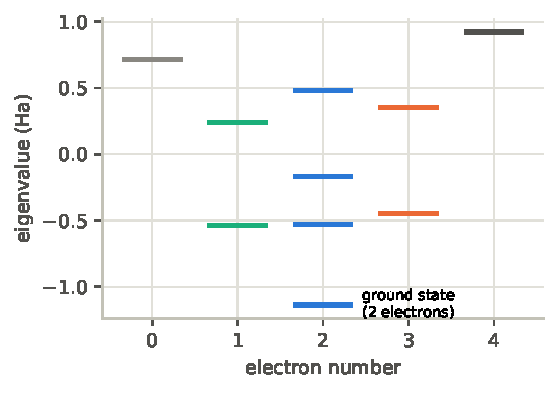
\includegraphics[width=\textwidth]{h2_spectrum}
    \end{column}
    \begin{column}{0.48\textwidth}
      \begin{itemize}
        \item All 16 eigenvalues of the notebook's 4-qubit H$_2$ Hamiltonian, sorted by electron number.
        \item The global minimum $\numfci$ Ha has exactly \key{2 electrons} --- the neutral molecule.
        \item Exact ground state: $0.9937\ket{1100} - 0.1125\ket{0011}$, i.e.\ $98.7\,\%$ Hartree--Fock, $1.3\,\%$ doubly excited.
        \item Excited states are $\ge 0.53$ Ha higher: VQE only needs the bottom.
      \end{itemize}
    \end{column}
  \end{columns}
\end{frame}

% =====================================================================================
\section{Part 3: From fermions to qubits}
\begin{frame}{Jordan--Wigner transformation}
  One qubit per spin-orbital; $\ket1$ = occupied, $\ket0$ = empty.
  \begin{block}{Mapping}
    \[ a_j^\dagger = Z_0Z_1\cdots Z_{j-1}\;\tfrac12(X_j - iY_j), \qquad n_j = \tfrac12(I - Z_j) \]
  \end{block}
  \begin{columns}[T]
    \begin{column}{0.5\textwidth}
      \begin{itemize}
        \item $\tfrac12(X - iY) = \ket1\bra0$ fills the orbital.
        \item The \key{$Z$-string} supplies the sign $(-1)^{n_0 + \dots + n_{j-1}}$ that makes operators on different orbitals \emph{anti}commute.
        \item Example: $a_2^\dagger = \tfrac12 Z_0Z_1(X_2 - iY_2)$ on 4 qubits.
      \end{itemize}
    \end{column}
    \begin{column}{0.46\textwidth}
      \begin{exampleblock}{Hopping term}
        $a_0^\dagger a_1 + a_1^\dagger a_0 = \tfrac12(X_0X_1 + Y_0Y_1)$\\[1mm]
        Derivation: $a_1 = Z_0\tfrac12(X_1 + iY_1)$, $(X - iY)Z = X - iY$, so $a_0^\dagger a_1 = \tfrac14(X_0 - iY_0)(X_1 + iY_1)$; adding the
        conjugate cancels the imaginary parts.
      \end{exampleblock}
      \small Weight of $a_j^\dagger$: $j + 1$, i.e.\ $O(N)$.
    \end{column}
  \end{columns}
\end{frame}

\begin{frame}{Bravyi--Kitaev, parity mapping and tapering}
  \begin{columns}[T]
    \begin{column}{0.52\textwidth}
      \begin{itemize}
        \item \key{Parity mapping}: qubit $j$ stores $n_0 \oplus \dots \oplus n_j$; occupations become non-local instead.
        \item \key{Bravyi--Kitaev}: qubits store partial sums on a binary tree: $b = Bn \bmod 2$. Both occupation and parity
          need only $O(\log N)$ qubits. E.g.\ $a_7^\dagger$ on 8 modes: weight 8 (JW) vs.\ 4 (BK).
        \item \key{Tapering}: $\mathbb Z_2$ symmetries (electron-number and spin parity) remove qubits exactly; H$_2$: 4 $\to$ 2 qubits.
      \end{itemize}
    \end{column}
    \begin{column}{0.44\textwidth}
      \begin{exampleblock}{BK on 4 modes}
        $B = \begin{psmallmatrix}1&0&0&0\\1&1&0&0\\0&0&1&0\\1&1&1&1\end{psmallmatrix}$\\[1mm]
        HF occupation $n = (1,1,0,0)$ $\to$ $b = (1, 0, 0, 0)$: the same physical state is $\ket{1100}$ in JW but $\ket{1000}$ in BK
        (checked: $\braket{1000|H_{\mathrm{BK}}|1000} = E_{\mathrm{HF}}$).
      \end{exampleblock}
      \small \texttt{VQE.ipynb} uses neither mapping explicitly: its H$_2$ coefficients are already Jordan--Wigner.
    \end{column}
  \end{columns}
\end{frame}

\begin{frame}{The notebook's H$_2$ qubit Hamiltonian}
  \small
  \begin{columns}[T]
    \begin{column}{0.5\textwidth}
      \begin{center}
      \begin{tabular}{lr}
        \toprule Pauli string & coefficient (Ha)\\ \midrule
        \texttt{IIII} & $-0.097066$\\
        \texttt{ZIII}, \texttt{IZII} & $+0.171413$\\
        \texttt{IIZI}, \texttt{IIIZ} & $-0.223432$\\
        \texttt{ZZII} & $+0.168689$\\
        \texttt{ZIZI}, \texttt{IZIZ} & $+0.120625$\\
        \texttt{ZIIZ}, \texttt{IZZI} & $+0.165928$\\
        \texttt{IIZZ} & $+0.174413$\\
        \texttt{XXYY}, \texttt{YYXX} & $-0.045303$\\
        \texttt{XYYX}, \texttt{YXXY} & $+0.045303$\\ \bottomrule
      \end{tabular}
      \end{center}
    \end{column}
    \begin{column}{0.46\textwidth}
      \begin{itemize}
        \item 15 terms; qubits = spin-orbitals $(\sigma_g\alpha, \sigma_g\beta, \sigma_u\alpha, \sigma_u\beta)$, STO-3G, Jordan--Wigner.
        \item \texttt{IIII} contains the nuclear repulsion and other constants.
        \item $Z$ terms: orbital energies and Coulomb/exchange between occupations. $XY$ terms: the double excitation $\ket{1100} \leftrightarrow \ket{0011}$.
      \end{itemize}
      \begin{alertblock}{Verified provenance}
        PySCF + OpenFermion reproduce all 15 coefficients to $\numcoefdiff$ at bond length \hl{$R = 0.740$ \AA}; the notebook's text says
        $0.7414$ \AA, where the coefficients differ by up to $1.8$ mHa.
      \end{alertblock}
    \end{column}
  \end{columns}
\end{frame}

\begin{frame}{Pauli decomposition of any Hamiltonian}
  \begin{columns}[T]
    \begin{column}{0.5\textwidth}
      The $4^n$ Pauli strings form an orthogonal basis of $2^n\times2^n$ matrices: $\operatorname{tr}(PQ) = 2^n\delta_{PQ}$. Hence
      \[ H = \sum_P c_PP,\qquad c_P = 2^{-n}\operatorname{tr}(PH) \in \mathbb R . \]
      \begin{exampleblock}{Worked example}
        $\begin{psmallmatrix}3 & 1 - 2i\\ 1 + 2i & -1\end{psmallmatrix} = I + X + 2Y + 2Z$\\[1mm]
        $\operatorname{diag}(1,2,3,4) = 2.5\,II - ZI - 0.5\,IZ$
      \end{exampleblock}
    \end{column}
    \begin{column}{0.46\textwidth}
      \centering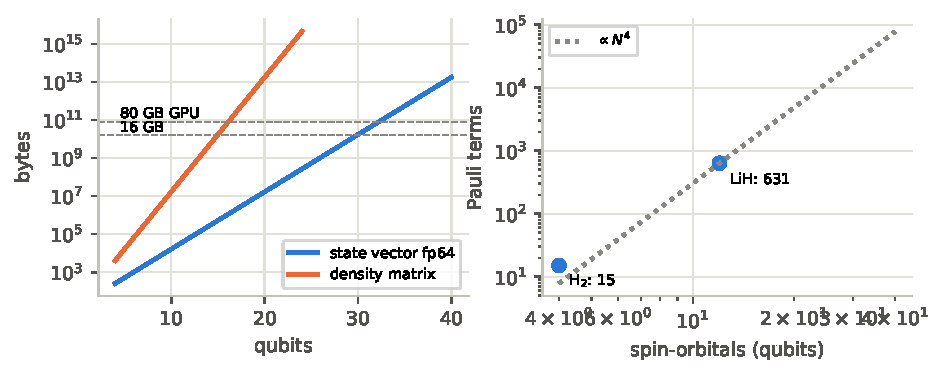
\includegraphics[width=\textwidth]{scaling}\\
      \small Left: memory of the state. Right: Pauli terms grow like $N^4$ --- H$_2$ 15, LiH (STO-3G, 12 qubits, generated with
      PySCF) 631. Illustrative; LiH is not in the notebook.
    \end{column}
  \end{columns}
\end{frame}

% =====================================================================================
\section{Part 4: The qubit toolkit}
\begin{frame}{Qubits, rotations and Pauli algebra}
  \begin{columns}[T]
    \begin{column}{0.5\textwidth}
      \begin{itemize}
        \item $\ket\psi = a\ket0 + b\ket1$; Born rule $P(0) = |a|^2$.
        \item Bloch vector $(\braket X, \braket Y, \braket Z)$.
        \item $R_Y(\theta) = e^{-i\theta Y/2}$: $R_Y(\theta)\ket0 = \cos\frac\theta2\ket0 + \sin\frac\theta2\ket1$ --- real amplitudes, Bloch vector $(\sin\theta, 0, \cos\theta)$.
        \item $e^{i\theta P} = \cos\theta\,I + i\sin\theta\,P$ for every Pauli string ($P^2 = I$).
      \end{itemize}
    \end{column}
    \begin{column}{0.46\textwidth}
      \begin{block}{Pauli algebra}
        $XY = iZ$, $YZ = iX$, $ZX = iY$; reversed order $\to$ minus sign.\\
        Strings multiply qubit by qubit: $(X\otimes Y)(Y\otimes X) = (iZ)\otimes(-iZ) = Z\otimes Z$.\\
        Two strings commute iff they anticommute at an \emph{even} number of positions.
      \end{block}
      \small Example: $X_0X_1X_2Y_3\ket{1100} = i\ket{0011}$ (two electrons moved).
    \end{column}
  \end{columns}
\end{frame}

\begin{frame}{Measuring a Pauli string}
  \begin{columns}[T]
    \begin{column}{0.5\textwidth}
      Hardware measures only $Z$. Rotate each factor first:
      \begin{center}\small
      \begin{tabular}{ll}
        \toprule factor & gates before $Z$-measurement\\ \midrule
        $X$ & $H$\\ $Y$ & $S^\dagger$, then $H$\\ $Z$ & none\\ $I$ & ignore the qubit\\ \bottomrule
      \end{tabular}
      \end{center}
      Each shot gives bits $b$; the outcome of $P$ is $(-1)^{\sum_{k\in\mathrm{supp}P}b_k}$; the average estimates $\braket P$ with
      standard error $\le 1/\sqrt S$.
    \end{column}
    \begin{column}{0.46\textwidth}
      \begin{block}{Grouping}
        Commuting strings share an eigenbasis and can use the same shots.
        \begin{itemize}
          \item \key{qubit-wise commuting} (QWC): same letter or $I$ at each position --- single-qubit rotations suffice.
          \item H$_2$: all $Z$ terms = 1 group; the 4 $XY$ terms commute but are not QWC: 5 settings (QWC) or 2 (general).
        \end{itemize}
      \end{block}
      \small On simulators \texttt{cudaq.observe} computes $\braket H$ exactly; with \texttt{shots\_count} it samples.
    \end{column}
  \end{columns}
\end{frame}

\begin{frame}{Expectation values: a numerical example}
  \begin{columns}[T]
    \begin{column}{0.52\textwidth}
      $H = 0.5\,Z_0 - 0.3\,Z_1 + 0.2\,X_0X_1$; measured $\braket{Z_0} = 0.6$, $\braket{Z_1} = -0.2$, $\braket{X_0X_1} = 0.5$:
      \[ E = 0.5(0.6) - 0.3(-0.2) + 0.2(0.5) = 0.46 . \]
      \begin{exampleblock}{Bell state $\frac{1}{\sqrt2}(\ket{00} + \ket{11})$}
        $\braket{ZZ} = 1$, $\braket{XX} = 1$, $\braket{YY} = -1$, $\braket{X_0} = \braket{X_1} = 0$.\\
        For $H = -Z_0Z_1 - \frac12(X_0 + X_1)$: $E = -1$, while $E_0 = -\sqrt2$.
      \end{exampleblock}
    \end{column}
    \begin{column}{0.44\textwidth}
      \begin{block}{Energy variance}
        $\mathrm{Var}(H) = \braket{H^2} - \braket H^2$ is zero exactly for eigenstates (zero-variance principle) and sets the shot noise
        $\sqrt{\mathrm{Var}/S}$.\\
        $H = -Z + \frac12X$: $H^2 = \frac54I$; $\mathrm{Var} = 0.25$ in $\ket0$, $0$ in the ground state.
      \end{block}
    \end{column}
  \end{columns}
\end{frame}

% =====================================================================================
\section{Part 5: The VQE algorithm}
\begin{frame}{The variational principle}
  \begin{columns}[T]
    \begin{column}{0.52\textwidth}
      \begin{block}{Theorem}
        For every normalised $\ket\psi$: \ $E[\psi] = \braket{\psi|H|\psi} \ge E_0$.
      \end{block}
      \textbf{Proof.} Expand in the eigenbasis, $\ket\psi = \sum_kc_k\ket{E_k}$, $\sum|c_k|^2 = 1$:
      \[ \braket{\psi|H|\psi} = \sum_k|c_k|^2E_k \ge \sum_k|c_k|^2E_0 = E_0 . \]
      Equality iff $\ket\psi$ is a ground state. Holds for mixed states too: $\operatorname{tr}(\rho H) \ge E_0$.
    \end{column}
    \begin{column}{0.44\textwidth}
      \centering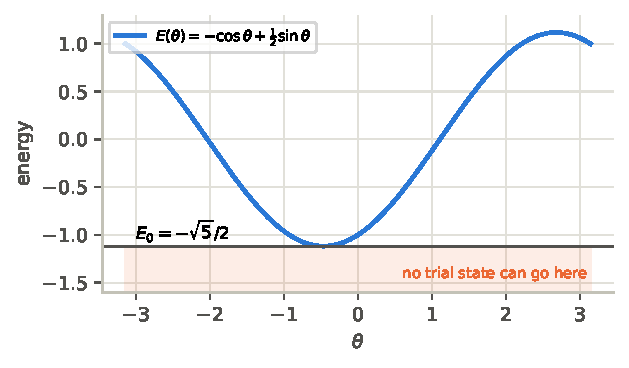
\includegraphics[width=\textwidth]{variational}\\
      \small One qubit, $H = -Z + \frac12X$, trial $R_Y(\theta)\ket0$: every trial energy lies above $E_0$; the minimum touches it at
      $\theta^* = -\arctan\frac12$.
    \end{column}
  \end{columns}
\end{frame}

\begin{frame}{Rayleigh--Ritz and what ``variational'' buys}
  \begin{columns}[T]
    \begin{column}{0.5\textwidth}
      \begin{block}{Rayleigh--Ritz}
        Diagonalise $H$ inside an $m$-dimensional trial space: the Ritz values satisfy $\varepsilon_k \ge E_{k-1}$ (upper bounds to the lowest
        $m$ exact levels). Larger spaces can only lower them.
      \end{block}
      \begin{itemize}
        \item VQE: the trial space is the set of states a circuit $U(\bt)$ can make --- curved, not linear.
        \item An energy \hl{below} $E_0$ with exact expectation values = a bug.
        \item With shots, single estimates can fall below by noise.
      \end{itemize}
    \end{column}
    \begin{column}{0.46\textwidth}
      \begin{alertblock}{Error is linear in contamination}
        $90\,\%$ ground state ($-1.13728$) + $10\,\%$ excited ($-0.53821$): $E = -1.0774$ Ha, error $59.9$ mHa.\\
        A good energy does not guarantee an equally good state.
      \end{alertblock}
    \end{column}
  \end{columns}
\end{frame}

\begin{frame}{The VQE loop}
  \begin{columns}[c]
    \begin{column}{0.5\textwidth}
      \centering
      \resizebox{\textwidth}{!}{%
      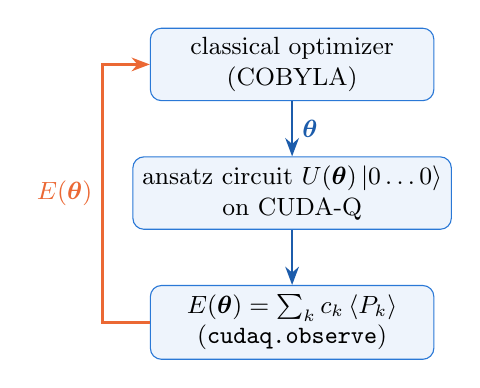
\begin{tikzpicture}[node distance=7mm, every node/.style={font=\small},
          box/.style={draw=qblue, fill=qlight, rounded corners, align=center, minimum width=36mm, minimum height=9mm}]
        \node[box] (opt) {classical optimizer\\(COBYLA)};
        \node[box, below=of opt] (qpu) {ansatz circuit $U(\bt)\ket{0\dots0}$\\on CUDA-Q};
        \node[box, below=of qpu] (obs) {$E(\bt) = \sum_kc_k\braket{P_k}$\\(\texttt{cudaq.observe})};
        \draw[-{Stealth}, thick, qdark] (opt) -- node[right] {$\bt$} (qpu);
        \draw[-{Stealth}, thick, qdark] (qpu) -- (obs);
        \draw[-{Stealth}, thick, qorange] (obs.west) -- ++(-6mm,0) |- node[pos=0.25, left] {$E(\bt)$} (opt.west);
      \end{tikzpicture}}
    \end{column}
    \begin{column}{0.46\textwidth}
      \begin{enumerate}
        \item Prepare $\ket{\psi(\bt)} = U(\bt)\ket{0\dots0}$ (normalised automatically: gates are unitary).
        \item Estimate $E(\bt)$ term by term.
        \item The optimizer proposes new $\bt$.
        \item Repeat until converged or the budget is used.
        \item Report the lowest energy seen and its angles.
      \end{enumerate}
      \small Quantum part: short circuits. Classical part: optimisation. Good for noisy hardware.
    \end{column}
  \end{columns}
\end{frame}

\begin{frame}{Ansatz design: three families}
  \small
  \begin{center}
  \begin{tabular}{p{2.6cm}p{4.1cm}p{4.1cm}p{3.2cm}}
    \toprule & \textbf{Chemically motivated (UCC)} & \textbf{Hardware-efficient (HEA)} & \textbf{Adaptive}\\ \midrule
    idea & $e^{T - T^\dagger}$ on top of Hartree--Fock & layers of native rotations + entanglers & grow the circuit operator by operator\\
    parameters & one per excitation ($O(N^4)$ for UCCSD) & $(L+1)N$ in the notebook & few, chosen by gradients\\
    depth & deep (Pauli gadgets, Trotter) & shallow, hardware-friendly & moderate\\
    symmetries & conserves electron number & usually not & by construction\\
    trainability & good start (HF), structured & barren plateaus when deep/random & good\\
    in the notebook & \texttt{ucc\_ansatz} (H$_2$) & \texttt{hea\_ansatz} (default) & --- \\ \bottomrule
  \end{tabular}
  \end{center}
  The ansatz decides what VQE can reach: the best VQE energy is $\min_{\bt}E(\bt)$ over the circuit's states, not $E_0$.
\end{frame}

\begin{frame}[fragile]{The Hartree--Fock reference state}
  \begin{columns}[T]
    \begin{column}{0.5\textwidth}
      \begin{itemize}
        \item The best single determinant: fill the lowest $N_e$ spin-orbitals.
        \item Under Jordan--Wigner it is a computational basis state: H$_2$ $\to$ $\ket{1100}$.
        \item Prepared with $X$ gates; energy $\braket{1100|H|1100} = \numehf$ Ha (only the identity and $Z$ terms contribute).
        \item It is the natural starting point ($\theta = 0$) of a chemistry VQE.
      \end{itemize}
    \end{column}
    \begin{column}{0.46\textwidth}
      \centering
      \begin{quantikz}[row sep=0.3cm, column sep=0.35cm]
        \lstick{$q_0\ (\sigma_g\alpha)$} & \gate{X} & \gate[4]{e^{i\theta X_0X_1X_2Y_3}} & \qw\\
        \lstick{$q_1\ (\sigma_g\beta)$} & \gate{X} & & \qw\\
        \lstick{$q_2\ (\sigma_u\alpha)$} & \qw & & \qw\\
        \lstick{$q_3\ (\sigma_u\beta)$} & \qw & & \qw
      \end{quantikz}\\[2mm]
      \small The notebook's UCC circuit: HF preparation, then one Pauli exponential (\texttt{exp\_pauli}).
    \end{column}
  \end{columns}
\end{frame}

\begin{frame}{Unitary coupled cluster (UCC)}
  \begin{columns}[T]
    \begin{column}{0.52\textwidth}
      \[ \ket{\psi} = e^{T - T^\dagger}\ket{\mathrm{HF}},\quad T = \sum_{ia}t_i^aa_a^\dagger a_i + \sum_{ijab}t_{ij}^{ab}a_a^\dagger a_b^\dagger a_ja_i \]
      ($i, j$ occupied, $a, b$ virtual).
      \begin{itemize}
        \item $T - T^\dagger$ is anti-Hermitian $\Rightarrow$ $e^{T - T^\dagger}$ unitary (classical CC uses non-unitary $e^T$).
        \item Count (spin-orbitals): singles $n_on_v$, doubles $\binom{n_o}{2}\binom{n_v}{2}$. LiH STO-3G: 32 + 168; H$_2$: 4 + 1.
        \item Under Jordan--Wigner one double excitation = 8 commuting Pauli strings, coefficients $\pm i/8$.
        \item Non-commuting excitations: Trotterise.
      \end{itemize}
    \end{column}
    \begin{column}{0.44\textwidth}
      \begin{block}{The notebook's shortcut for H$_2$}
        Keep one string: $\ket{\psi(\theta)} = e^{i\theta X_0X_1X_2Y_3}\ket{1100}$. Since $X_0X_1X_2Y_3\ket{1100} = i\ket{0011}$,
        \[ \ket{\psi(\theta)} = \cos\theta\ket{1100} - \sin\theta\ket{0011} . \]
        Exact for H$_2$: the ground state lies in this plane (singles vanish by symmetry).
      \end{block}
    \end{column}
  \end{columns}
\end{frame}

\begin{frame}[fragile]{The hardware-efficient ansatz (default)}
  \centering
  \resizebox{0.92\textwidth}{!}{%
  \begin{quantikz}[row sep=0.25cm, column sep=0.25cm]
    \lstick{$q_0$} & \gate{R_Y(\theta_0)} & \ctrl{1} & \qw & \qw & \gate{R_Y(\theta_4)} & \ctrl{1} & \qw & \qw & \gate{R_Y(\theta_8)} & \qw\\
    \lstick{$q_1$} & \gate{R_Y(\theta_1)} & \targ{} & \ctrl{1} & \qw & \gate{R_Y(\theta_5)} & \targ{} & \ctrl{1} & \qw & \gate{R_Y(\theta_9)} & \qw\\
    \lstick{$q_2$} & \gate{R_Y(\theta_2)} & \qw & \targ{} & \ctrl{1} & \gate{R_Y(\theta_6)} & \qw & \targ{} & \ctrl{1} & \gate{R_Y(\theta_{10})} & \qw\\
    \lstick{$q_3$} & \gate{R_Y(\theta_3)} & \qw & \qw & \targ{} & \gate{R_Y(\theta_7)} & \qw & \qw & \targ{} & \gate{R_Y(\theta_{11})} & \qw
  \end{quantikz}}\\[3mm]
  \raggedright\small
  \begin{itemize}
    \item $L$ layers of [$R_Y$ on every qubit, CNOT ladder $q\to q+1$] + final $R_Y$ layer (drawn: $N = 4$, $L = 2$).
    \item Parameters $(L+1)N$, CNOTs $L(N-1)$. Default $N = 15$, $L = 2$: \key{45 parameters, 28 CNOTs, 73 gates} (recorded statistics, depth 20).
    \item Only real gates $\Rightarrow$ real amplitudes: adequate because the Ising and H$_2$ Hamiltonians are real symmetric.
    \item Initial angles $\sim\mathcal N(0, 0.1^2)$ (seed 42): starts near $\ket{0\dots0}$, whose Ising energy is $-14$.
  \end{itemize}
\end{frame}

\begin{frame}{Classical optimizers and parameter updates}
  \begin{columns}[T]
    \begin{column}{0.52\textwidth}
      \small
      \begin{tabular}{p{1.8cm}p{4.6cm}}
        \toprule optimizer & principle (all in the notebook)\\ \midrule
        COBYLA & linear models in a trust region, derivative-free (default, \texttt{rhobeg = 0.3})\\
        Nelder--Mead & simplex of $n_p + 1$ points\\
        Powell & line searches along conjugate directions\\
        L-BFGS-B & quasi-Newton; finite-difference gradients ($n_p + 1$ runs each)\\ \bottomrule
      \end{tabular}
    \end{column}
    \begin{column}{0.44\textwidth}
      \begin{block}{Gradients on a quantum computer}
        For a gate $e^{-i\theta P/2}$: \ $\partial_\theta E = \tfrac12[E(\theta + \tfrac\pi2) - E(\theta - \tfrac\pi2)]$ --- exact
        (\key{parameter shift}). HEA default: $2\times45 = 90$ runs per gradient.
      \end{block}
      \small \key{Convergence}: COBYLA stops when its trust region shrinks below \texttt{tol} or when \texttt{maxiter} is reached;
      the notebook keeps the best energy of the whole history.
    \end{column}
  \end{columns}
\end{frame}

\begin{frame}[fragile]{VQE in pseudocode}
\begin{lstlisting}[language={}]
input : Hamiltonian H = sum_k c_k P_k (Pauli strings), ansatz U(theta), initial angles theta0
define energy(theta):
    prepare |psi(theta)> = U(theta)|0...0>                  # e.g. X X on q0,q1 + exp_pauli, or RY + CNOT layers
    E = 0
    for each group of commuting P_k:                         # simulator: exact; hardware: basis change + shots
        E += c_k * <psi(theta)| P_k |psi(theta)>
    return E
theta* <- classical_minimise(energy, theta0)               # COBYLA, MAX_EVALUATIONS = 300
report  min over all evaluated energies, its angles, |E - E0| if an exact E0 is known
sample  U(theta*)|0...0> to show the dominant bitstrings
\end{lstlisting}
  \small Every call of \texttt{energy} is one full quantum simulation (or a batch of hardware shots).
\end{frame}

% =====================================================================================
\section{Part 6: Worked examples}
\begin{frame}{H$_2$: VQE as a $2\times2$ eigenproblem}
  \begin{columns}[T]
    \begin{column}{0.52\textwidth}
      The UCC state lives in $\mathrm{span}\{\ket{1100}, \ket{0011}\}$. With $H_{11} = \braket{1100|H|1100}$, $H_{22} = \braket{0011|H|0011}$,
      $H_{12} = \braket{1100|H|0011}$:
      \[ E(\theta) = H_{11}\cos^2\theta + H_{22}\sin^2\theta - H_{12}\sin2\theta . \]
      \small
      $H_{11} = -1.116759$, $H_{22} = 0.462618$, $H_{12} = 0.181210$ Ha.\\
      $E'(\theta) = 0$: $\tan2\theta^* = \frac{2H_{12}}{H_{22} - H_{11}} = 0.2295$ $\Rightarrow$ $\theta^* = \numthetastar$.\\
      $E_{\min} = \frac{H_{11} + H_{22}}{2} - \sqrt{\left(\frac{H_{22} - H_{11}}{2}\right)^2 + H_{12}^2} = \numfci$ Ha.
    \end{column}
    \begin{column}{0.46\textwidth}
      \centering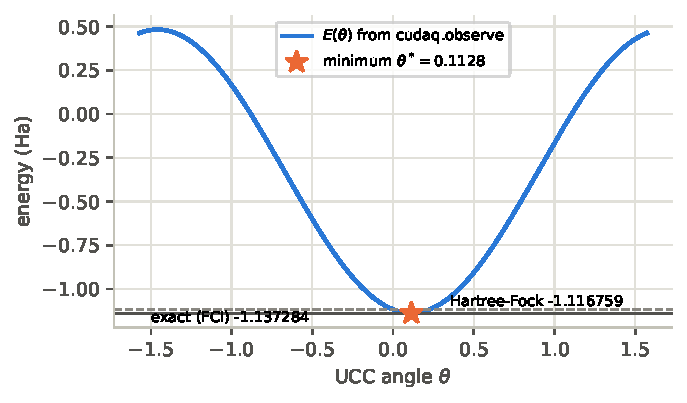
\includegraphics[width=\textwidth]{h2_landscape}\\
      \small CUDA-Q: $E(\theta^*) = \numeucc$ Ha, error $\numuccerr$ Ha vs.\ FCI; $P(\ket{0011}) = \numpdouble$.
    \end{column}
  \end{columns}
\end{frame}

\begin{frame}{H$_2$: the VQE loop and the dissociation curve}
  \begin{columns}[T]
    \begin{column}{0.48\textwidth}
      \centering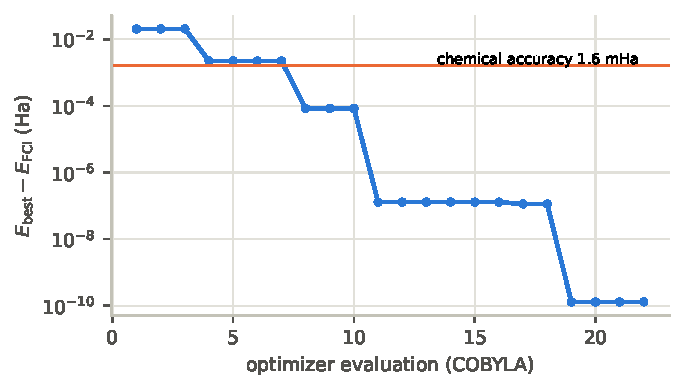
\includegraphics[width=\textwidth]{h2_convergence}\\
      \small Notebook settings (COBYLA from $\theta = 0$): chemical accuracy after \numhacc{} evaluations; best
      $\numhbest$ Ha after \numhevals{} evaluations (error $\numherr$ Ha).
    \end{column}
    \begin{column}{0.48\textwidth}
      \centering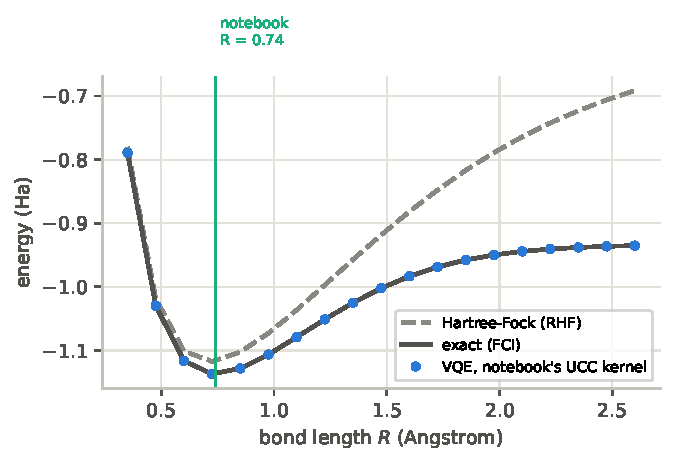
\includegraphics[width=\textwidth]{h2_dissociation}\\
      \small Illustrative scan (PySCF + OpenFermion Hamiltonians, the notebook's UCC kernel in CUDA-Q): VQE follows FCI (max deviation
      $\numvqemaxdev$ Ha); RHF fails at large $R$ ($\numhfgapfar$ mHa too high at $2.6$ \AA).
    \end{column}
  \end{columns}
\end{frame}

\begin{frame}{Two-qubit Ising chain by hand}
  \begin{columns}[T]
    \begin{column}{0.52\textwidth}
      $H = -Z_0Z_1 - \frac12(X_0 + X_1)$. Circuit: $R_Y(\theta_0)$, $R_Y(\theta_1)$, CNOT$_{0\to1}$.
      \begin{enumerate}
        \item $\theta_0 = \frac\pi2$, $\theta_1 = 0$: Bell state; $E = -1$.
        \item Exact: $H$ commutes with $X_0X_1$; in the block $\{\ket{\Phi^+}, \ket{\Psi^+}\}$: $\begin{psmallmatrix}-1&-1\\-1&1\end{psmallmatrix}$, so $E_0 = -\sqrt2$.
        \item Relative error of the Bell state: $29.3\,\%$.
        \item In general $\braket{Z_0Z_1} = \cos\theta_1$ after the CNOT (Heisenberg: CNOT maps $Z_0Z_1 \to Z_1$).
      \end{enumerate}
    \end{column}
    \begin{column}{0.44\textwidth}
      \begin{block}{Free-fermion reference}
        The notebook maps the open chain to free fermions: a $2N\times2N$ antisymmetric matrix $A$,
        $E_0 = -\tfrac12\sum|\lambda(iA)|$. $N = 2$: $-\sqrt2$; $N = 15$: $\numtfeo$; $N = 100$: a $200\times200$ matrix.
      \end{block}
    \end{column}
  \end{columns}
\end{frame}

% =====================================================================================
\section{Part 7: CUDA-Q implementation}
\begin{frame}{The structure of \texttt{VQE.ipynb}}
  \begin{columns}[T]
    \begin{column}{0.5\textwidth}
      \footnotesize
      \begin{enumerate}\itemsep0pt
        \item Problem statement and mathematics
        \item Imports and version check
        \item \key{Input parameters} (the only cell to edit)
        \item Hamiltonian, validation, exact reference
        \item Benchmark utilities, backend selection
        \item Expected output: memory, time estimate
        \item Ansatz kernels, drawing, statistics, QIR export
        \item \key{Execution}: VQE loop + final sampling, memory monitor
        \item Convergence, error and bitstring plots
        \item Final benchmark report (\texttt{exports/vqe/})
      \end{enumerate}
    \end{column}
    \begin{column}{0.46\textwidth}
      \begin{block}{Section 3 defaults}
        \small
        \texttt{HAMILTONIAN = "tfim"}, \texttt{N\_QUBITS = 15}, \texttt{TFIM\_J = 1.0}, \texttt{TFIM\_H = 0.5}\\
        \texttt{ANSATZ = "auto"} (UCC for H$_2$, HEA otherwise), \texttt{ANSATZ\_LAYERS = 2}, \texttt{INITIAL\_PARAMETER\_SCALE = 0.1}\\
        \texttt{OPTIMIZER = "COBYLA"}, \texttt{MAX\_EVALUATIONS = 300}, \texttt{OBJECTIVE\_SHOTS = None}\\
        \texttt{REFERENCE\_MAX\_QUBITS = 18}, \texttt{SHOTS = 4000}, \texttt{SEED = 42}
      \end{block}
      \small Options: \texttt{"H2"} (4 qubits) or \texttt{"custom"} (list of (coefficient, Pauli word)).
    \end{column}
  \end{columns}
\end{frame}

\begin{frame}[fragile]{Building the Hamiltonian and the exact reference (Section 4)}
\begin{lstlisting}
for i in range(n_qubits - 1):                     # -J Z_i Z_{i+1}
    word = ["I"] * n_qubits; word[i] = word[i + 1] = "Z"
    pauli_terms.append((-float(TFIM_J), "".join(word)))
for i in range(n_qubits):                         # -h X_i
    word = ["I"] * n_qubits; word[i] = "X"
    pauli_terms.append((-float(TFIM_H), "".join(word)))

def build_spin_operator(terms):                   # sum_k c_k P_k as a CUDA-Q SpinOperator
    operator = None
    for coefficient, word in terms:
        term = coefficient * cudaq.SpinOperator.from_word(word)   # character i acts on qubit i
        operator = term if operator is None else operator + term
    return operator

def tfim_exact_energy(n, J, h):                   # free fermions: E0 = -1/2 sum |eig(iA)|
    A = np.zeros((2 * n, 2 * n))
    ...                                           # -h X_j and -J Z_j Z_{j+1} as Majorana couplings
    return -0.5 * float(np.sum(np.abs(np.linalg.eigvalsh(1j * A))))
\end{lstlisting}
  \small Default: 29 terms (14 $ZZ$ + 15 $X$). Reference $E_0 = -15.0825179883$; sparse diagonalisation (cross-check for $N \le 16$) gives the same.
\end{frame}

\begin{frame}[fragile]{The ansatz kernels, line by line (Section 7a)}
  \begin{columns}[T]
    \begin{column}{0.58\textwidth}
\begin{lstlisting}
@cudaq.kernel
def hea_ansatz(n: int, layers: int, theta: list[float]):
    qubits = cudaq.qvector(n)              # |0...0>
    k = 0                                  # next angle
    for layer in range(layers):
        for q in range(n):
            ry(theta[k], qubits[q]); k += 1
        for q in range(n - 1):
            x.ctrl(qubits[q], qubits[q + 1])   # CNOT ladder
    for q in range(n):                     # final layer
        ry(theta[k], qubits[q]); k += 1

@cudaq.kernel
def ucc_ansatz(theta: list[float]):
    qubits = cudaq.qvector(4)
    x(qubits[0]); x(qubits[1])             # HF |1100>
    exp_pauli(theta[0], qubits, "XXXY")    # e^{i theta XXXY}
\end{lstlisting}
    \end{column}
    \begin{column}{0.40\textwidth}
      \small
      \begin{itemize}
        \item \texttt{@cudaq.kernel}: compiled to MLIR/QIR and JIT-compiled.
        \item \texttt{ry(t, q)} $= e^{-itY/2}$; \texttt{x.ctrl(c, t)} = CNOT.
        \item Angle order: layer by layer, qubit by qubit.
        \item \texttt{exp\_pauli(t, q, "XXXY")} $= e^{+itX_0X_1X_2Y_3}$ (sign verified in CUDA-Q 0.16): $\cos t\ket{1100} - \sin t\ket{0011}$.
        \item \texttt{*\_sampled} variants add \texttt{mz(qubits)}.
      \end{itemize}
    \end{column}
  \end{columns}
\end{frame}

\begin{frame}[fragile]{The energy function and the optimiser (Section 8)}
\begin{lstlisting}
def energy(theta):
    kernel, args = ansatz_call(kernels, theta)                 # HEA or UCC with its arguments
    result = cudaq.observe(kernel, hamiltonian, *args, **observe_kwargs)   # exact, or shots_count=...
    value = result.expectation()                               # E(theta) = sum_k c_k <P_k>
    energy_history.append(value); theta_history.append(np.array(theta, dtype=float))
    return value

opt = minimize(energy, initial_theta, method="COBYLA", options={"maxiter": MAX_EVALUATIONS, "rhobeg": 0.3})
best_index = int(np.argmin(energy_history))                    # best evaluated, not necessarily opt.x
best_theta, vqe_energy = theta_history[best_index], energy_history[best_index]
final_counts = cudaq.sample(kernel_s, *args_s, shots_count=SHOTS)   # dominant bitstrings
\end{lstlisting}
  \begin{itemize}\small
    \item Printed results: optimizer message, VQE energy, reference, absolute and relative error; for H$_2$ ``Chemical accuracy (1.6 mHa): REACHED/not reached''.
    \item Plots: energy per evaluation and best-so-far, log error, dominant bitstrings, memory timeline.
  \end{itemize}
\end{frame}

\begin{frame}{CPU, GPU, multi-GPU and hardware}
  \small
  \begin{center}
  \resizebox{\textwidth}{!}{%
  \begin{tabular}{llll}
    \toprule \texttt{BACKEND} + \texttt{SIMULATION\_METHOD} & CUDA-Q target & memory & executed here?\\ \midrule
    \texttt{cpu} + \texttt{statevector} & \texttt{qpp-cpu} & $16\times2^n$ B & \textbf{yes}\\
    \texttt{cpu} + \texttt{density\_matrix} & \texttt{density-matrix-cpu} & $16\times4^n$ B & no\\
    \texttt{gpu} + \texttt{statevector} & \texttt{nvidia} (fp32/fp64) & $8$ / $16\times2^n$ B & no (no GPU)\\
    \texttt{gpu} + \texttt{mps} / \texttt{tensornet} & \texttt{tensornet-mps} / \texttt{tensornet} & entanglement-dependent & no (no GPU)\\
    \texttt{multi-gpu} + \texttt{statevector} & \texttt{nvidia}, option \texttt{mgpu} (MPI) & split over GPUs & no\\
    \texttt{hardware} & \texttt{quantinuum}, \texttt{ionq}, \dots & --- & no\\ \bottomrule
  \end{tabular}}
  \end{center}
  \begin{itemize}
    \item \texttt{"auto"}: GPU if visible, else CPU. An explicit \texttt{"gpu"} without a GPU raises a \texttt{RuntimeError} (never touches GPU targets).
    \item Multi-GPU pooling needs \texttt{mpiexec}, one rank per GPU. Hardware returns samples only: the energy is then always estimated from shots.
    \item Section 6 checks memory against \texttt{MEMORY\_SAFETY\_FRACTION} and prints a rough time estimate.
  \end{itemize}
\end{frame}

% =====================================================================================
\section{Part 8: Results}
\begin{frame}{Recorded, re-executed and lecture-script results (Ising chain)}
  \footnotesize
  \begin{center}
  \resizebox{0.95\textwidth}{!}{%
  \begin{tabular}{lccc}
    \toprule & \textbf{previously recorded} & \textbf{re-executed notebook} & \textbf{this lecture's script}\\ \midrule
    machine & 4 vCPU Xeon & laptop, WSL Ubuntu & laptop, WSL Ubuntu\\
    CUDA-Q / target & 0.16.0 / \texttt{qpp-cpu} & 0.16.0 / \texttt{qpp-cpu} & 0.16.0 / \texttt{qpp-cpu}\\
    evaluations & 300 (budget) & RERUNEVALS & \numtfevals\\
    $E_{\mathrm{VQE}}$ & $-15.0533898284$ & RERUNE & $\numtfbest$\\
    error vs.\ $E_0 = -15.0825179883$ & $2.913\times10^{-2}$ ($0.193\,\%$) & RERUNERR & $\numtferr$ ($\numtfrel\,\%$)\\
    $P(\ket{0\dots0})$ (4000 shots) & 0.7005 & RERUNPZERO & \numtfpzero\\
    execution cell / loop & 70.1 s & RERUNTIME & \numtftime{} s\\ \bottomrule
  \end{tabular}}
  \end{center}
  \begin{itemize}
    \item Same seed, same initial angles, same COBYLA settings; differences in the last digits come from floating-point summation order.
    \item Only the CPU state-vector path was executed; GPU, multi-GPU and hardware paths are implemented but \hl{not validated}.
  \end{itemize}
\end{frame}

\begin{frame}{Convergence of the default run}
  \centering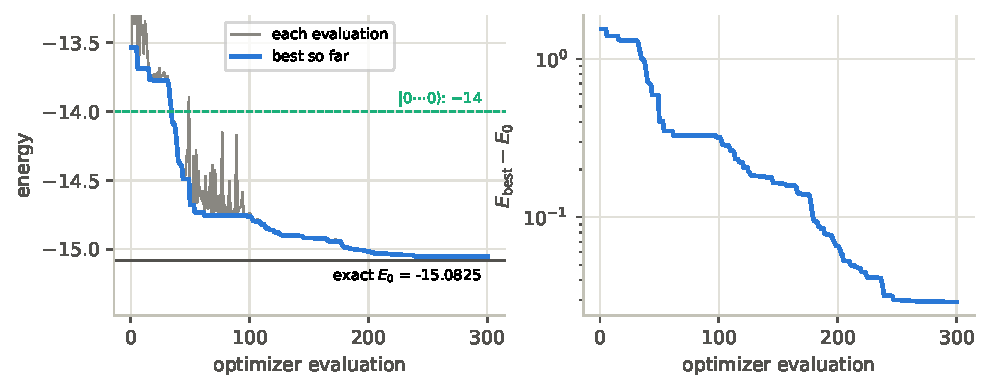
\includegraphics[width=0.88\textwidth]{tfim_convergence}\\
  \raggedright\footnotesize
  \begin{itemize}
    \item The first evaluation ($\numtfstart$) is near the product state $\ket{0\dots0}$ ($-14$); the curve approaches $E_0$ \key{from above}.
    \item The log-error plot is still falling at the end: COBYLA stopped because of the budget (\texttt{MAXFUN}), not because it converged.
  \end{itemize}
\end{frame}

\begin{frame}{Reading the Ising results}
  \begin{columns}[T]
    \begin{column}{0.5\textwidth}
      \begin{block}{Dominant bitstrings (this lecture's run)}
        \small
        \begin{tabular}{lr}
          \toprule bitstring (qubit 0 first) & probability\\ \midrule
          \numtftop
          \bottomrule
        \end{tabular}
      \end{block}
    \end{column}
    \begin{column}{0.46\textwidth}
      \small
      \begin{itemize}
        \item \key{Relative error} $0.193\,\%$ looks tiny, but the product state $\ket{0\dots0}$ already gives $-14$. Measured from there, VQE
          recovered $97.3\,\%$ of the remaining $1.0825$.
        \item \key{Symmetry breaking}: the exact ground state is symmetric under flipping all spins ($P(0\dots0) = P(1\dots1)$); the shallow ansatz
          settles on one branch, at an energy cost exponentially small in $N$.
        \item Next steps: more evaluations, then more layers (the notebook suggests 4 layers / 800 evaluations at $h = J$).
      \end{itemize}
    \end{column}
  \end{columns}
\end{frame}

\begin{frame}{Performance of the recorded run}
  \begin{columns}[T]
    \begin{column}{0.5\textwidth}
      \small
      \begin{center}
      \begin{tabular}{lr}
        \toprule phase (recorded) & time\\ \midrule
        circuit construction & 0.017 s\\
        compilation (MLIR + JIT) & 0.038 s\\
        quantum execution (300 \texttt{observe}) & 69.10 s\\
        final sampling (4000 shots) & 0.22 s\\
        optimizer + Python & 0.67 s\\ \midrule
        execution cell & 70.09 s\\ \bottomrule
      \end{tabular}
      \end{center}
    \end{column}
    \begin{column}{0.46\textwidth}
      \small
      \begin{itemize}
        \item $69.10/300 = 0.23$ s per energy evaluation (73-gate circuit, 29 terms, 15 qubits).
        \item Pre-run estimate $\sim102.9$ s: $1.5\times$ high, within the stated $\pm3\times$.
        \item State memory 524 kB; peak RAM 0.92 GB --- the runtime, not the state, dominates at 15 qubits.
        \item At 25--28 qubits each evaluation is $2^{10}$--$2^{13}\times$ costlier: the notebook suggests a GPU.
      \end{itemize}
    \end{column}
  \end{columns}
\end{frame}

% =====================================================================================
\section{Part 9: Shots, noise and hardware}
\begin{frame}{Measurement shots}
  \begin{columns}[T]
    \begin{column}{0.52\textwidth}
      \begin{itemize}
        \item Each estimated $\braket{P_k}$ has standard error $\le 1/\sqrt{S}$; the energy combines them with weights $c_k$.
        \item Per-shot spread $\sigma$ of the energy estimator $\Rightarrow$ $S = (\sigma/\varepsilon)^2$ shots for precision $\varepsilon$.
          $\sigma = 0.1$ Ha, $\varepsilon = 1.6$ mHa: $\approx 3.9\times10^3$ shots \emph{per energy evaluation}.
        \item Grouping commuting terms and allocating shots by $|c_k|$ reduce the cost.
        \item With shots, single evaluations can dip below $E_0$ --- the notebook's text warns about this.
      \end{itemize}
    \end{column}
    \begin{column}{0.44\textwidth}
      \begin{block}{In the notebook}
        \texttt{OBJECTIVE\_SHOTS = None}: exact energies (simulators). An integer: \texttt{cudaq.observe(..., shots\_count=n)}.
        Hardware: always shots (\texttt{SHOTS}).
      \end{block}
      \small Try \texttt{OBJECTIVE\_SHOTS = 2000}: the convergence curve becomes noisy, as on a real device.
    \end{column}
  \end{columns}
\end{frame}

\begin{frame}{Noise, error mitigation and hardware}
  \begin{columns}[T]
    \begin{column}{0.5\textwidth}
      \footnotesize
      \begin{itemize}
        \item Noise turns pure states into mixtures; the variational bound still holds ($\operatorname{tr}\rho H \ge E_0$), but energies rise.
        \item Complete depolarisation: $E = \operatorname{tr}H/2^n = c_{I\dots I} = -0.0971$ Ha for H$_2$.
        \item Illustrative global-depolarising model: $E(p) = (1 - p)E_{\mathrm{FCI}} + p\,c_{IIII}$; already $p = \numpbreakeven$ loses the whole correlation energy.
        \item \key{Error mitigation}: zero-noise extrapolation ($E(\lambda{=}1) = -1.10$, $E(3) = -1.00$ $\Rightarrow$ $E(0) \approx -1.15$; no variational guarantee),
          readout correction, symmetry verification (electron number).
        \item \key{Hardware}: limited connectivity (SWAPs), native gates, CNOT errors $10^{-3}$--$10^{-2}$: shallow ansätze preferred.
      \end{itemize}
    \end{column}
    \begin{column}{0.46\textwidth}
      \centering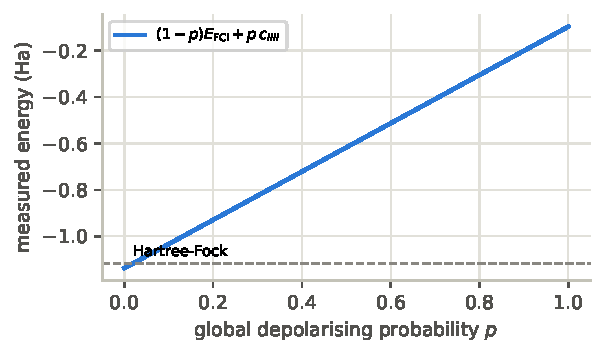
\includegraphics[width=\textwidth]{noise_model}\\
      \small Model for illustration, not a hardware measurement; \texttt{Noise\_Simulation.ipynb} shows CUDA-Q noise channels.
    \end{column}
  \end{columns}
\end{frame}

% =====================================================================================
\section{Part 10: Limits and outlook}
\begin{frame}{Limitations}
  \begin{columns}[T]
    \begin{column}{0.5\textwidth}
      \small
      \begin{itemize}
        \item \key{Measurement cost}: $O(N^4)$ terms, $(\sigma/\varepsilon)^2$ shots each evaluation, hundreds of evaluations.
        \item \key{Barren plateaus}: for deep random (hardware-efficient) circuits the gradient variance decays exponentially with $n$.
        \item \key{Local minima} and optimizer budgets (the default run stopped at its budget).
        \item \key{Expressiveness}: the result is only as good as the ansatz; shallow HEA misses correlations, deep UCC is long.
        \item \key{Noise} raises energies; mitigation costs more shots.
      \end{itemize}
    \end{column}
    \begin{column}{0.46\textwidth}
      \begin{block}{Honest status}
        \small No quantum advantage for chemistry has been demonstrated with VQE. Classical methods (CCSD(T), DMRG) handle molecules far
        beyond today's devices. VQE's value today: a well-understood hybrid algorithm and a benchmark; the notebook reproduces small
        problems exactly on a simulator.
      \end{block}
    \end{column}
  \end{columns}
\end{frame}

\begin{frame}{Advanced VQE and applications}
  \footnotesize
  \begin{columns}[T]
    \begin{column}{0.5\textwidth}
      \begin{block}{Better ansätze and fewer qubits}
        \begin{itemize}
          \item \key{ADAPT-VQE}: add operators one by one from a pool, chosen by energy gradient.
          \item \key{k-UpCCGSD}, qubit-coupled cluster: cheaper chemistry-inspired circuits.
          \item \key{Active spaces}, frozen core (LiH: 12 $\to$ 10 qubits), tapering.
        \end{itemize}
      \end{block}
      \begin{block}{Excited states}
        Variational quantum deflation (penalise overlap with found states), subspace-search VQE, quantum subspace expansion.
      \end{block}
    \end{column}
    \begin{column}{0.46\textwidth}
      \begin{block}{Applications}
        \begin{itemize}
          \item reaction energies and barriers; catalysts
          \item potential energy surfaces (bond breaking)
          \item battery and photovoltaic materials (lattice models, Hubbard)
          \item magnetism: spin chains such as the notebook's Ising model
        \end{itemize}
      \end{block}
      None of the advanced variants is implemented in \texttt{VQE.ipynb}.
    \end{column}
  \end{columns}
\end{frame}

\begin{frame}{Try it yourself: \texttt{VQE.ipynb}}
  \begin{columns}[T]
    \begin{column}{0.5\textwidth}
      \begin{enumerate}
        \item \texttt{pip install -r requirements.txt}, open \texttt{VQE.ipynb}, run all cells.
        \item Edit only Section 3:
          \begin{itemize}
            \item \texttt{HAMILTONIAN = "H2"}: UCC, chemical accuracy in a few evaluations
            \item \texttt{TFIM\_H = 1.0}: the critical point, much harder
            \item \texttt{ANSATZ\_LAYERS = 4}, \texttt{MAX\_EVALUATIONS = 800}
          \end{itemize}
      \end{enumerate}
    \end{column}
    \begin{column}{0.46\textwidth}
      \begin{block}{Experiments}
        \begin{itemize}
          \item \texttt{OBJECTIVE\_SHOTS = 2000}: optimise with shot noise
          \item \texttt{OPTIMIZER = "L-BFGS-B"}: gradient-based
          \item \texttt{HAMILTONIAN = "custom"} with your own Pauli words
          \item \texttt{N\_QUBITS = 24}, \texttt{BACKEND = "gpu"}: timing on a GPU
        \end{itemize}
      \end{block}
    \end{column}
  \end{columns}
\end{frame}

% =====================================================================================
\section{Part 11: Practice and summary}
\begin{frame}{Exercises}
  \begin{enumerate}
    \item Eigenvalues and ground-state vector of $\begin{psmallmatrix}0 & 1\\ 1 & 0\end{psmallmatrix}$; Rayleigh quotient of $(1, 0)$.
    \item Decompose $\operatorname{diag}(2, 0, 0, -2)$ into Pauli strings.
    \item Write $a_1^\dagger$ on 3 qubits under Jordan--Wigner.
    \item Compute $X_0Y_1\ket{00}$ and $\braket{00|X_0X_1|00}$.
    \item For $H = Z + X$ and trial $R_Y(\theta)\ket0$: $E(\theta)$, $\theta^*$ and $E_0$.
    \item Parameters, CNOTs and gates of the notebook's HEA for $N = 6$, $L = 3$.
    \item An energy estimator has $\sigma = 0.05$ Ha. Shots for a standard error of $1$ mHa?
    \item Why can a VQE energy computed with exact expectation values never be below $E_0$?
  \end{enumerate}
\end{frame}

\begin{frame}{Answers}
  \small
  \begin{enumerate}
    \item $\pm1$; ground state $\frac{1}{\sqrt2}(1, -1)$; $R((1, 0)) = 0 \ge -1$.
    \item $\operatorname{diag}(2, 0, 0, -2) = Z_0 + Z_1$ (check $\ket{11}$: $-1 - 1 = -2$).
    \item $a_1^\dagger = Z_0\,\tfrac12(X_1 - iY_1)\otimes I_2$.
    \item $X_0Y_1\ket{00} = \ket1\otimes i\ket1 = i\ket{11}$; $\braket{00|X_0X_1|00} = \braket{00|11} = 0$.
    \item $E = \cos\theta + \sin\theta = \sqrt2\sin(\theta + \frac\pi4)$; $\theta^* = -\frac{3\pi}{4}$; $E_0 = -\sqrt2$.
    \item $(3 + 1)\cdot6 = 24$ parameters, $3\cdot5 = 15$ CNOTs, $39$ gates.
    \item $S = (0.05/0.001)^2 = 2500$.
    \item The circuit state is normalised and $\braket{\psi|H|\psi} = \sum_k|c_k|^2E_k \ge E_0$ (variational principle).
  \end{enumerate}
\end{frame}

\begin{frame}{Summary}
  \begin{columns}[T]
    \begin{column}{0.56\textwidth}
      \footnotesize
      \begin{itemize}\itemsep1pt
        \item Ground-state energies are eigenvalue problems of exponentially large Hermitian matrices.
        \item Molecules: Born--Oppenheimer $\to$ second quantisation $\to$ Jordan--Wigner/Bravyi--Kitaev $\to$ $H = \sum_kc_kP_k$ with $O(N^4)$ terms.
        \item \key{Variational principle}: $\braket{\psi|H|\psi} \ge E_0$ --- VQE minimises the energy of a circuit state.
        \item Ansätze: Hartree--Fock + UCC (exact for H$_2$ with one parameter), or hardware-efficient $R_Y$ + CNOT layers.
        \item Energies are measured term by term; shots and noise dominate the cost on hardware.
        \item \texttt{VQE.ipynb}: Ising chain within $0.193\,\%$ of the exact $E_0$ (budget-limited); H$_2$ reaches FCI --- reproduced here with CUDA-Q.
      \end{itemize}
    \end{column}
    \begin{column}{0.40\textwidth}
      \begin{block}{Further reading}
        \scriptsize
        \begin{itemize}\itemsep0pt
          \item A.\ Peruzzo et al., \emph{A variational eigenvalue solver on a photonic quantum processor}, Nat.\ Commun.\ 5 (2014)
          \item J.\ McClean et al., \emph{The theory of variational hybrid quantum-classical algorithms}, NJP 18 (2016)
          \item A.\ Kandala et al., \emph{Hardware-efficient VQE for small molecules}, Nature 549 (2017)
          \item J.\ Tilly et al., \emph{The Variational Quantum Eigensolver: a review}, Phys.\ Rep.\ 986 (2022)
          \item NVIDIA CUDA-Q documentation
          \item This repository: \texttt{VQE.ipynb}, \texttt{assessments/VQE\_*.pdf}
        \end{itemize}
      \end{block}
    \end{column}
  \end{columns}
\end{frame}

\end{document}
